%
% quotient.tex
%
% (c) 2021 Prof Dr Andreas Müller, OST Ostschweizer Fachhochschule
%
\bgroup
\definecolor{darkred}{rgb}{0.7,0,0}
\definecolor{darkgreen}{rgb}{0,0.6,0}
\def\s{0.3}
\def\punkt#1#2{({#1-3*#2},{8*#2})}
\def\gerade#1{
\draw[darkgreen,line width=1.4pt]
	\punkt{#1}{1}
	--
	\punkt{#1}{-1};
}
\begin{frame}[t]
\setlength{\abovedisplayskip}{5pt}
\setlength{\belowdisplayskip}{5pt}
\frametitle{Quotientenraum}
\vspace{-18pt}
\begin{columns}[t,onlytextwidth]
\begin{column}{0.48\textwidth}
\begin{block}{Einen Unterraum ``ignorieren''}
{\usebeamercolor[fg]{title}Gegeben:} $U\subset V$ ein Unterraum
\\
{\usebeamercolor[fg]{title}Gesucht:} Eine Projektion auf einen Vektorraum,
in dem die Richtungen in $U$ zu $0$ gemacht werden
\end{block}
\uncover<2->{%
\begin{block}{Projektion}
In $V$ Klassen bilden:
\[
\pi
\colon
v\mapsto
\llbracket v\rrbracket
=
v+U
\]
\end{block}}
\vspace{-12pt}
\uncover<3->{%
\begin{block}{Quotientenraum}
\vspace{-12pt}
\begin{align*}
V/U
&=
\{ v+U\;|\; v\in V \}
\\
\uncover<4->{\pi(\lambda v)&=\lambda v+U= \lambda \pi(v)}
\\
\uncover<5->{\pi(v+w)
&=
v+w+U}
\ifthenelse{\boolean{presentation}}{
\only<6>{=
v+U+w+U}}{}
\uncover<7->{=
\pi(v) + \pi(w)}
\phantom{blubb}
\end{align*}
\end{block}}
\end{column}
\begin{column}{0.48\textwidth}
\begin{center}
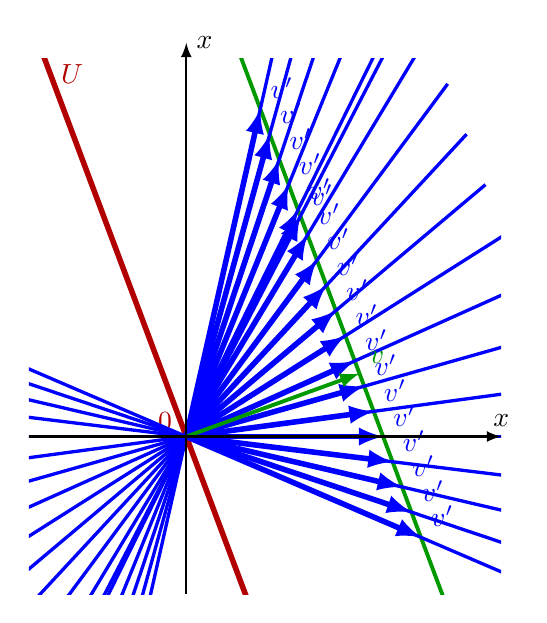
\begin{tikzpicture}[>=latex,thick]
\coordinate (U) at (-3,8);
\def\t{0.03}
\begin{scope}
\clip (-2,-2) rectangle (4,4.8);
\draw[color=darkred,line width=2pt] (-3,8) -- (1.5,-4);
\node[color=darkred] at (-1.45,4.6) {$U$};
\node[color=darkred] at (-0.05,-0.05) [above left] {$0$};

\gerade{2.5}

\ifthenelse{\boolean{presentation}}{
	\foreach \n in {8,...,25}{
		\pgfmathparse{(\n-12)*0.04}
		\xdef\s{\pgfmathresult}
		\only<\n>{
			\draw[color=blue,line width=1.2pt]
				\punkt{-5}{-2*\s} -- \punkt{5}{2*\s};
			\draw[->,color=blue,line width=2pt]
				(0,0) -- \punkt{2.5}{\s};
			\node[color=blue] at \punkt{2.5}{\s}
				[above right] {$v'$};
		}
	}
}{
	\xdef\s{0.35}
	\draw[color=blue,line width=1.2pt]
		\punkt{-5}{-2*\s} -- \punkt{5}{2*\s};
	\draw[->,color=blue,line width=2pt] (0,0) -- \punkt{2.5}{\s};
	\node[color=blue] at \punkt{2.5}{\s} [above right] {$v'$};
}

\draw[->,color=darkgreen,line width=1.4pt] (0,0) -- \punkt{2.5}{0.1};

\node[color=darkgreen] at \punkt{2.5}{0.1} [above right] {$v$};

\end{scope}
\draw[->] (-2,0) -- (4,0) coordinate[label={$x$}];
\draw[->] (0,-2) -- (0,5) coordinate[label={right:$x$}];
\end{tikzpicture}
\end{center}
\end{column}
\end{columns}
\end{frame}
